\documentclass{beamer}
\usepackage{tikz}

\usepackage[latin1]{inputenc}

% Makes new math operators
\usepackage{microtype}  %This gives MUCH better PDF results!
\usepackage{fnbreak} %warn for split footnotes
\usepackage{booktabs} %nice tables
\usepackage{tabularx}
\usepackage{amsopn}
\usepackage{amsmath}
\usepackage{amsfonts}
\usepackage{graphicx}
\usepackage{pgf}
\usepackage{tikz}
\usepackage{url}
\usepackage{comment}
\usepackage{todonotes}
\usepackage{algpseudocode}
\usepackage{algorithm}
\usepackage{bm}
\usepackage{url}
\usepackage{hyperref}

\usetikzlibrary{arrows,positioning}
\tikzset{
    >=stealth',
    bigPunkt/.style={
           rectangle,
           rounded corners,
           draw=black, very thick,
           text width=6.5em,
           minimum height=10em,
           text centered},
    punkt/.style={
           rectangle,
           rounded corners,
           draw=black, very thick,
           text width=6.5em,
           minimum height=5em,
           text centered},
    pil/.style={
           ->,
           thick,
           shorten <=2pt,
           shorten >=2pt,}
}
\newcommand{\isFalse}{\ensuremath{\mathsf{isFalse}}}
\newcommand{\isUndef}{\ensuremath{\mathsf{isUndef}}}
\newcommand{\isTrue}{\ensuremath{\mathsf{isUndef}}}
\newcommand{\isSet}{\ensuremath{\mathsf{isSet}}}
\newcommand{\canBeTrue}{\ensuremath{\mathsf{canBeTrue}}}
\newcommand{\canBeFalse}{\ensuremath{\mathsf{canBeFalse}}}
\newcommand{\canBeUndef}{\ensuremath{\mathsf{canBeUndef}}}


\usetheme{Boadilla}
\title{Leveraging GPUs for Effective Clause Sharing in Parallel SAT Solving}
\author{Nicolas Prevot, Mate Soos, and Kuldeep S. Meel}
\date{\today}

\begin{document}
\begin{frame}
\titlepage
\end{frame}

\begin{frame}
\frametitle{Parallel SAT solving approaches}
\begin{itemize}
\item Divide and conquer
\begin{itemize}
\item Separate the search spaces between threads
\end{itemize}
\item Portfolio approach
\begin{itemize}
\item Different parameters for different threads
\item Threads share some clauses
\item This is our approach
\end{itemize}
\end{itemize}
\end{frame}

\begin{frame}
\frametitle{Clause exchange}
\begin{itemize}
\item Sharing too many clauses leads to a slowdown
\item We need to identify good clause and only share those
\item Clauses with a small size/lbd are usually better
\item Some state-of-the-are solvers share only clauses with small size or lbd
\end{itemize}
\end{frame}

\begin{frame}
\frametitle{Our approach}
\begin{itemize}
\item We can measure a clause usefulness by how often it is used
\item Clauses that have been used are more likely to be used again
\item Identify clauses which would have been used recently, import those
\end{itemize}
\end{frame}

\begin{frame}
\frametitle{Identifying clauses which would have been used}
\begin{itemize}
\item SAT solvers perform propagation until completion, or they reach a conflict
\item Consider assignments where unit propagation completed without conflict
\item Indentify clauses which would have been used on those (in conflict or implying)
\end{itemize}
\end{frame}

\begin{frame}
\frametitle{Example of used clauses}
\begin{itemize}
\item Thread completes propagation with: $v_1 \leftarrow F, v_2 \leftarrow F$
\begin{itemize}
\item Clause $v_1 \lor v_2 \lor v_3$ would have implied $ v_3 \leftarrow T$
\item Clause $v_1 \lor v_2$ would have been in conflict
\item Clause $\neg v_1 \lor v_2$ would not have told us anything new
\end{itemize}
\item We say a clause triggers an assignment if it would have implied something or been in conflict
\end{itemize}
\end{frame}

\begin{frame}
\frametitle{Architecture}
\begin{figure}[htb]
	\centering
\scalebox{0.64}{
	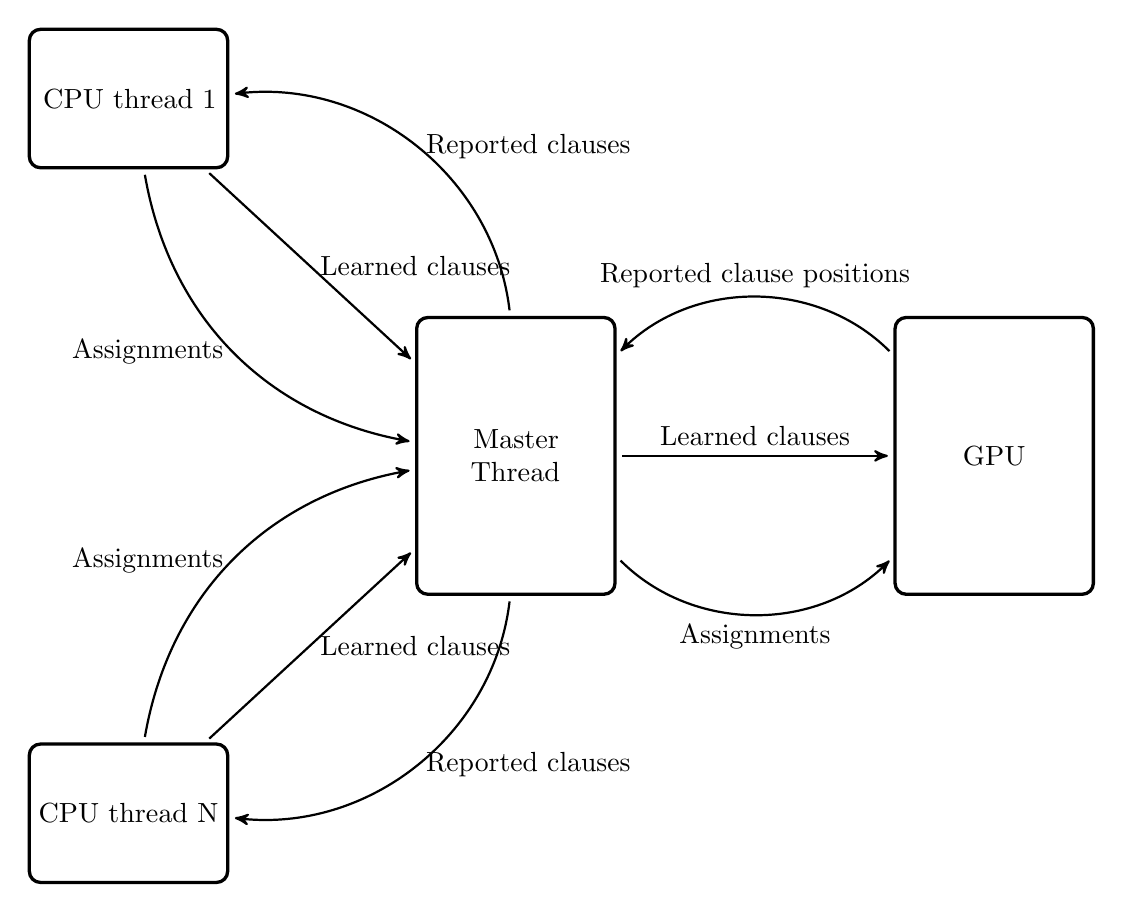
\begin{tikzpicture}[node distance=1cm, auto]
	\node (Dummy){};
	\node[punkt, above = 10em of Dummy] (CPUThread1) {CPU thread 1};
	\node[punkt, below = 10em of Dummy] (CPUThread2) {CPU thread N};
	\node[bigPunkt, right = 10em of Dummy] (MasterThread) {Master Thread};
	\node[bigPunkt, right = 10em of  MasterThread] (GPU) {GPU};
	\draw [pil, bend right=45, midway, right] (MasterThread) edge node{Reported clauses} (CPUThread1);
	\draw [pil, midway, right] (CPUThread1) edge node{Learned clauses} ({MasterThread});
	\draw [pil, bend right=35, midway, left] (CPUThread1) edge node{Assignments} (MasterThread);
	\draw [pil, bend left=35, midway, left] (CPUThread2) edge node{Assignments} (MasterThread);
	\draw [pil, midway, right] (CPUThread2) edge node{Learned clauses} (MasterThread);
	\draw [pil, bend left=45, midway, right] (MasterThread) edge node{Reported clauses} (CPUThread2);
	\draw [pil, bend right=45, midway, above] (GPU) edge node{Reported clause positions} (MasterThread);
	\draw [pil] (MasterThread) edge node{Learned clauses} (GPU);
	\draw [pil, bend right=45, midway, below] (MasterThread) edge node{Assignments} (GPU);
	\end{tikzpicture}
}
\end{figure}

\end{frame}

\begin{frame}
\frametitle{Bitwise representation of assignments}

\begin{center}
\begin{tabular}{ | c | c | c |}
\hline
 & $v_1$ & $v_2$ \\ 
\hline
assignment A & T & U \\  
assignment B & U & F \\    
\hline
isSet & 10 & 01 \\
isTrue & 10 & 00 \\
\hline
\end{tabular}
\end{center}
\end{frame}

\begin{frame}
\frametitle{Testing a clause on 32 assignments}

\begin{algorithm}[H]
\begin{algorithmic}[1]
    \State $\mathsf{allFalse} \gets [1,\cdots 1]$ \Comment{bit-vector of size $k$ with each bit initialized to 1}
    \State $\mathsf{oneUndef} \gets [0, \cdots, 0]$ \Comment{bit-vector of size $k$ with each bit initialized to 0}
    \For {$\ell \in \mathsf{cl}$}
        \State $\mathsf{oneUndef} \gets (\mathsf{allFalse} \& \isUndef(\bm{\mathcal{A}}(\ell))) \mid  (\mathsf{oneUndef} \& \isFalse(\bm{\mathcal{A}}(\ell)))$
        \State $\mathsf{allFalse} \gets \mathsf{allFalse} \& \isFalse(\bm{\mathcal{A}}(\ell))$
    \EndFor
    \State  $\mathsf{res} \gets \mathsf{oneUndef} \mid  \mathsf{allFalse}$
    \State \Return $\mathsf{res}$
\end{algorithmic}
\end{algorithm}

\end{frame}

\begin{frame}
\frametitle{Group testing}
\begin{itemize}
\item Testing a clause on 32 assignments at once still isn't fast enough
\item Group assignments by the solver thread they come from
\item Test a clause on the groups first, only test it on individual assignments if it's positive
\end{itemize}
\end{frame}

\begin{frame}
\frametitle{Pooled assignment}
\begin{center}
\begin{tabular}{ | c | c | c | c |}
\hline
 & $v_1$ & $v_2$ & $v_3$\\ 
\hline
assignment A & T & F & U \\  
assignment B & U & F & F \\    
\hline
pooled assignment & \{T, U \} & \{F\} & \{U, F\}\\
\hline
\end{tabular}
\end{center}
\end{frame}

\begin{frame}
\frametitle{Clause triggering a pooled assignment}
\begin{definition}
	A clause $\mathsf{cl}$ of size s triggers on an pooled assignment $P$ if both of the following conditions hold true:
	\begin{enumerate}
		\item For each literal $\ell$ in $\mathsf{cl}$, $P(\ell) \cap \{U,F\} \neq \emptyset$
		\item For at least s - 1 literals $\ell \in \mathsf{cl}$, $F \in P(\ell)$
	\end{enumerate}
\end{definition}
If a clause does not trigger on a pooled assignment, it does not trigger on any of the associated assignments
\end{frame}

\begin{frame}
\frametitle{Bitwise representation of pooled assignments}
\begin{center}
\begin{tabular}{ | c | c | c |}
\hline
 & $v_1$ & $v_2$ \\ 
\hline
pooled assignment A & \{T, U\} & \{U\} \\  
pooled assignment B & \{U\} & \{T, F, U\} \\    
\hline
canBeTrue & 10 & 01 \\
canBeFalse & 00 & 01 \\
canBeUndef & 11 & 11 \\
\hline
\end{tabular}
\end{center}

With this representation, we can test a clause on up to 32 pooled assignments at once.
\end{frame}

\begin{frame}
\frametitle{overall clause testing}
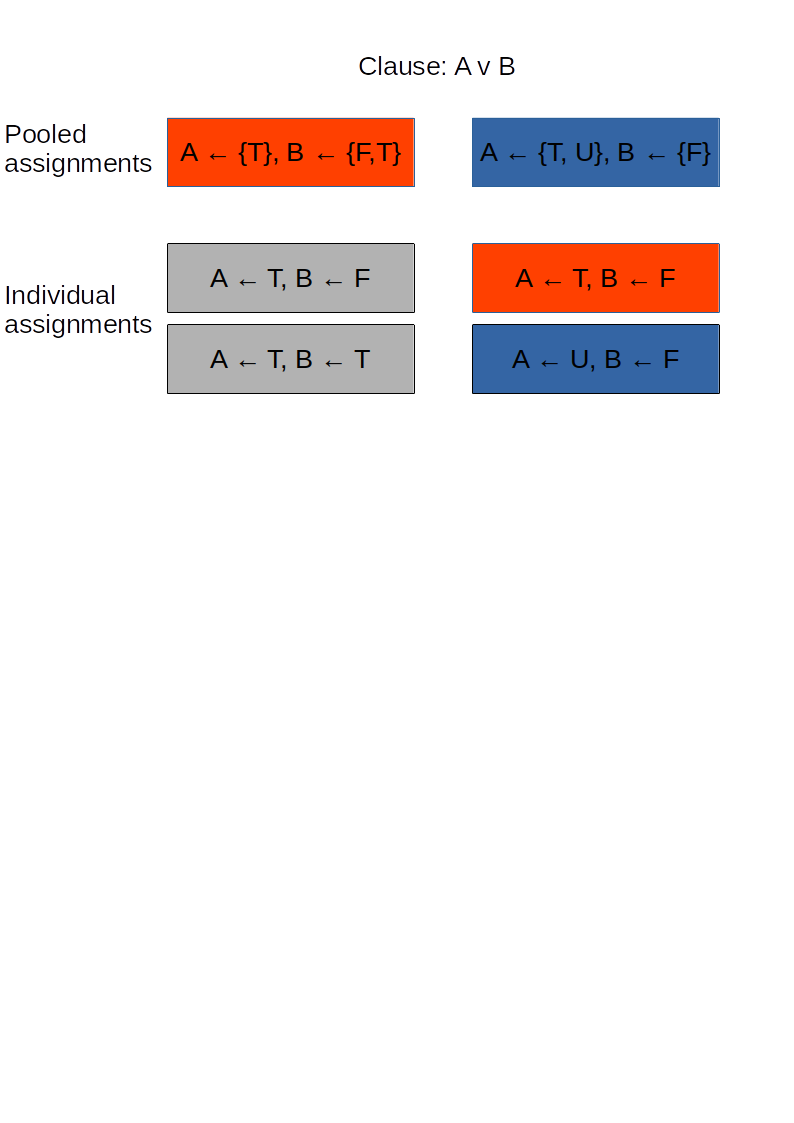
\includegraphics[width=\textwidth]{clauseTest.png}
\end{frame}

\begin{frame}
\frametitle{Comparison with glucose-syrup}
\begin{figure}[h]
	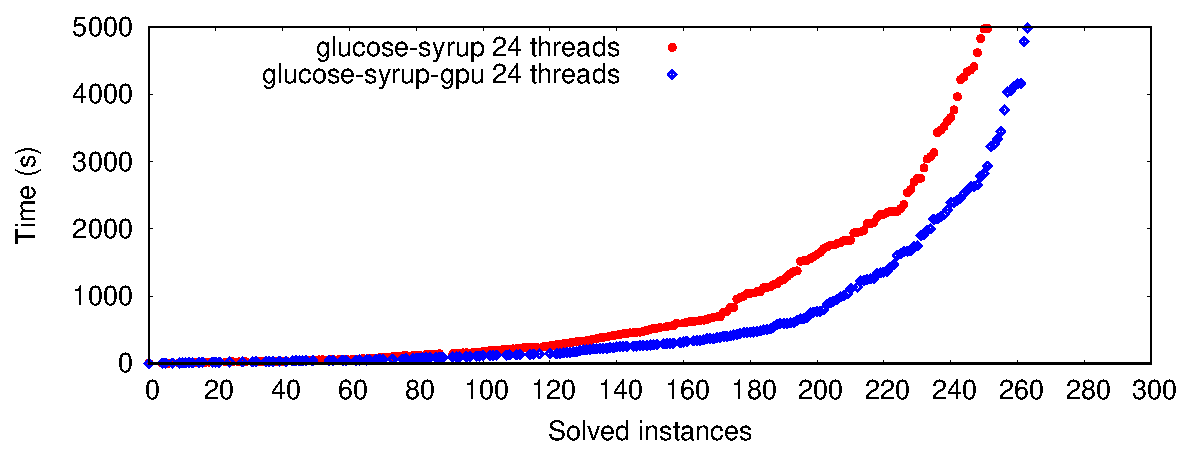
\includegraphics[width=\textwidth]{cactusplot_syrup_vs_syrup_gpu}
	\caption{glucose-syrup vs glucose-syrup + GpuShareSat. glucose-syrup solved 124 SAT and 127 UNSAT instances. glucose-syrup-gpu solved 132 SAT and 131 UNSAT instances.  }
	\label{cactus:syrup}
\end{figure}
\end{frame}

\begin{frame}
\frametitle{Comparison with P-MCOMSPS-STR}
\begin{figure}[htb]
	\centering
	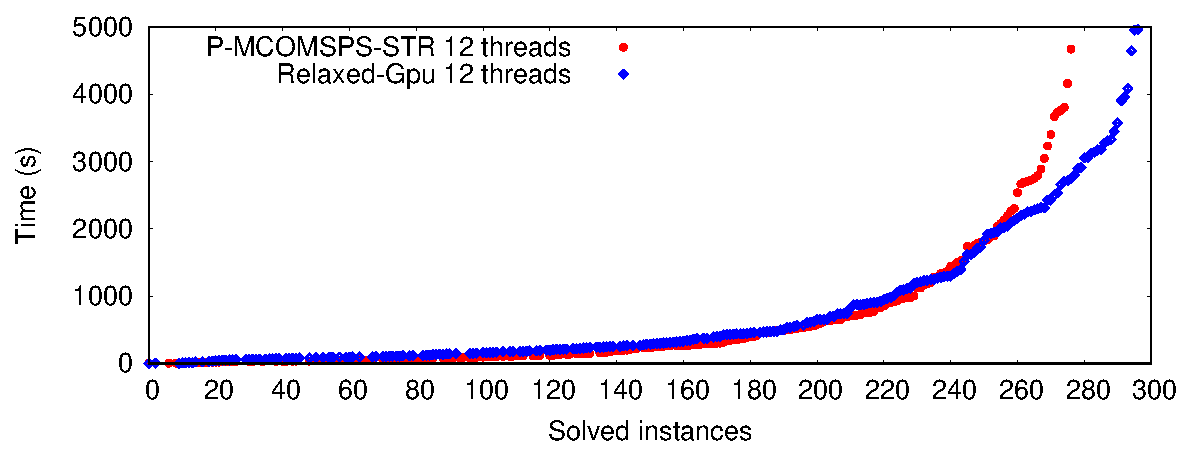
\includegraphics[width=\textwidth]{cactusplot_painless_vs_relaxed_gpu}
	\caption{P-MCOMSPS-STR vs Relaxed\_LCMDCBDL\_newTech + GpuShareSat}
	\label{cactus:relaxed}
\end{figure}
\begin{itemize}
\item P-MCOMSPS-STR came first in sat 2020 parallel competition
\item Relaxed\_LCMDCBDL\_newTech came third in sat 2020 single threaded competition
\end{itemize}
\end{frame}

\end{document}

